\documentclass[12pt,a4paper]{article}

% ============================================
% PACKAGES
% ============================================

\usepackage{mathptmx}
\usepackage[T1]{fontenc}
\usepackage{setspace}
\doublespacing
\usepackage[margin=2.54cm]{geometry}
\usepackage{amsmath}
\usepackage{amssymb}
\usepackage{graphicx}
\usepackage{booktabs}
\usepackage{makecell}
\usepackage{natbib}
\bibliographystyle{apalike}
\usepackage{hyperref}
\hypersetup{hidelinks}

% ============================================
% DOCUMENT
% ============================================

\begin{document}

% ============================================
% TITLE PAGE
% ============================================

\begin{titlepage}
    \centering
    \vspace*{2cm}
    {\Large\bfseries Gender Pricing and Service Duration: Evidence from European Salons\par}
    \vspace{1.5cm}
    \begin{flushleft}
    \textbf{Richard Schulz}\\
    Albert Einstein School of Public Policy\\
    Department of Humanities, Social and Political Sciences, D-GESS\\
    ETH Zürich\\
    Email: rschul@ethz.ch\\
    ORCID: \href{https://orcid.org/0009-0007-9702-9211}{0009-0007-9702-9211}\\
    Corresponding author: Richard Schulz\\
    \vfill
\textbf{Word Count:} 1,878 (main text, references, and captions)
    \end{flushleft}
    \vfill
\end{titlepage}

\newpage

% ============================================
% ABSTRACT
% ============================================

\begin{center}
    \textbf{Abstract}
\end{center}

\noindent
I examine how prices for women's and men's haircuts vary with appointment length across 33,682 listings from salons in ten European countries. Comparing a single average price for each gender obscures how salons structure their menus, since average duration differs by gender. Across all adult listings, women's haircuts cost €9.1 more on average. When comparing men's and women's haircuts of the exact same listed duration within the same salon, the difference is €5.3. Within duration categories, the estimated gap is €3.6 for appointments up to 30 minutes, compared with €11.9 for appointments between 46 and 60 minutes. Because salons decide how much time to list for each service, my estimates only reflect posted menu prices and do not prove price discrimination.

\vspace{0.5cm}

\noindent
\textbf{Keywords:} gender pricing, haircut markets, service markets, posted prices

\noindent
\textbf{JEL Classifications:} D18, J16, L84, D40

\newpage

% ============================================
% MAIN TEXT
% ============================================

\section{Introduction}

In product markets, detailed analyses find that cost differences rather than markups explain observed gender price gaps, consistent with the ease of arbitrage in posted-price retail \citep{moshary2023gender, barnesbrounstein2024}. Service markets differ because consumers often cannot avoid a gender-coded service category by buying the version marketed to another gender. Gender price gaps in service markets have long been documented \citep{ukHairdressers, duesterhaus2011cost, Heiden2018-wc, Affairs2015FromCT}, but existing work typically treats the gap as a single average difference between male- and female-coded services. Focusing only on a single average obscures how salons structure their menus, since prices, durations, and gender labels are posted together and average duration differs by gender.

I use 33,682 haircut listings from 13,658 salons in ten European countries to examine how prices for women's and men's haircuts vary with listed appointment length. Across all adult listings, women's haircuts cost about €9.1 more on average. When comparing men's and women's haircuts of the exact same listed duration within the same salon, the difference is €5.3. Within duration categories, the estimated gap is €3.6 for appointments up to 30 minutes, compared with €11.9 for appointments between 46 and 60 minutes. The same-duration gap also remains positive and significant when restricting to male- and female-coded listings with identical service titles. Overall, my results show that price differences between men's and women's haircuts persist for identical time slots within the same salon and widen at longer appointment lengths.

\section{Empirical Framework and Data}

\subsection{Data}

The adult analysis sample contains 33,682 haircut listings from 13,658 salons in Austria, Belgium, France, Germany, Italy, the Netherlands, Portugal, Spain, Switzerland, and the United Kingdom, collected in June 2025 from a major European online booking platform. The sample is restricted to haircut listings, excluding bundled treatments such as coloring, perms, extensions, and beard work. Each listing records a service name, listed duration, price, and salon-provided platform gender category. Prices are converted to euros using OECD PPP data \citep{OECD_PPP_GDP}. In the adult analysis sample, male-coded listings average €24.5 and 34.27 listed minutes, while female-coded listings average €33.6 and 46.35 listed minutes.

The estimates describe posted adult haircut prices observed in June 2025. The within-salon regressions reported below are restricted to the 20,758 listings in the 6,459 unisex salons that list at least one male-coded and one female-coded adult haircut.

Figure~\ref{fig:duration_distribution} shows the marginal duration distributions in unisex salons. Male- and female-coded listings overlap at common durations such as 30, 45, and 60 minutes, while female-coded listings are more concentrated at longer durations. The within-salon comparisons below use salon-duration cells rather than only this marginal overlap.

\begin{figure}[htbp]
    \centering
    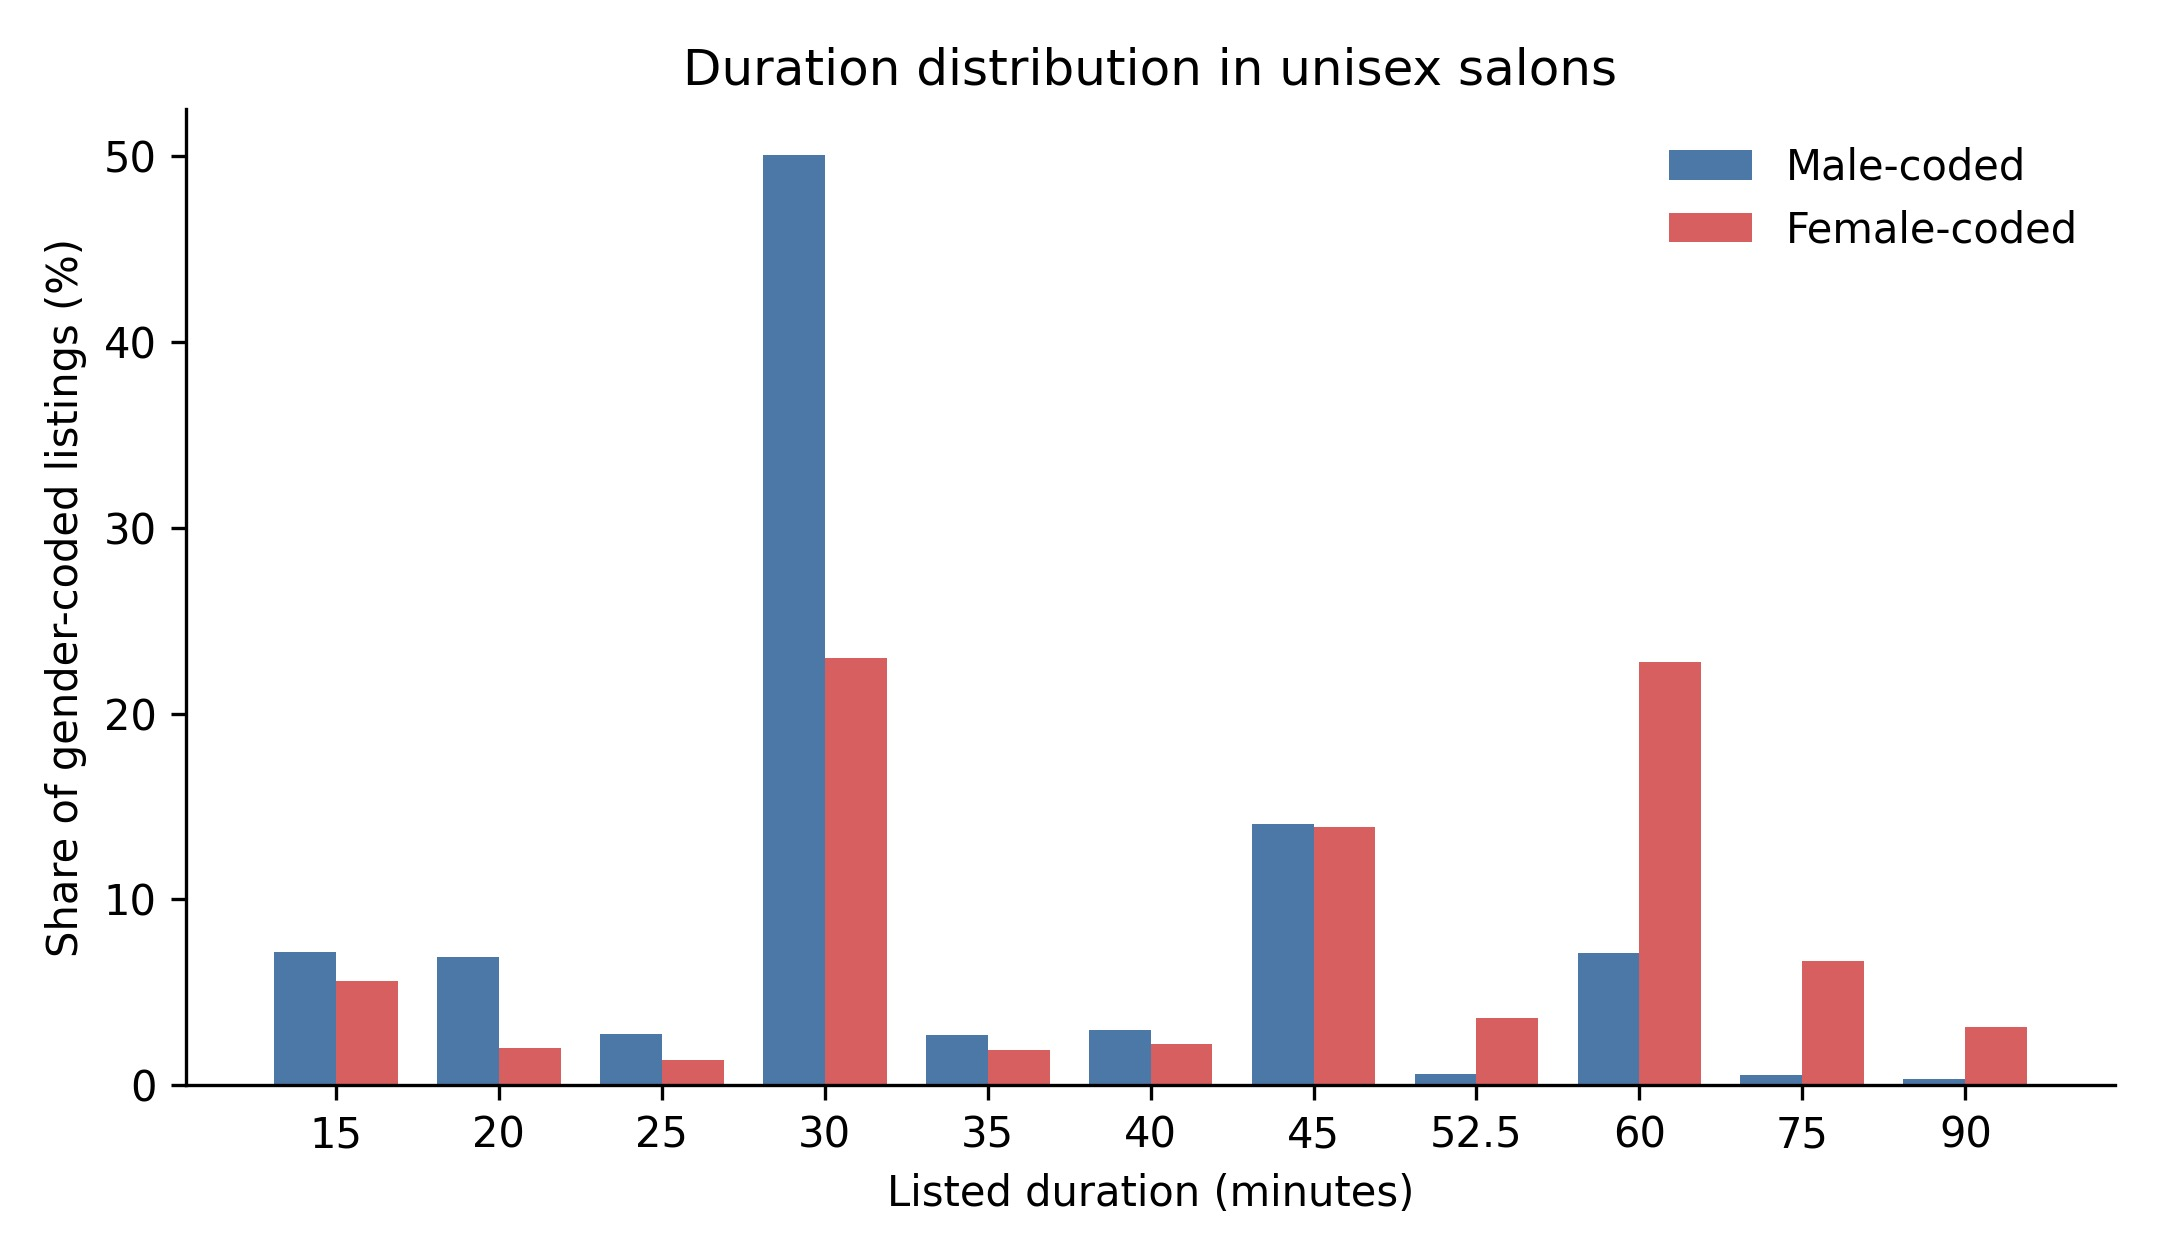
\includegraphics[width=0.82\linewidth]{figure_duration_distribution_by_gender.jpeg}
    \caption{Listed Duration Distribution by Gender in Unisex Salons}
    \label{fig:duration_distribution}
\end{figure}

\subsection{Empirical Strategy}

The first comparisons use only durations where male- and female-coded listings can be compared within the same salon. In salon-duration cells containing both male- and female-coded listings, I estimate
\[
\text{price}_{ijd} = \theta \cdot \text{female}_{ijd} + \delta_{jd} + \varepsilon_{ijd},
\]
where $\delta_{jd}$ is a salon-by-exact-duration fixed effect. This specification holds fixed both the salon and the exact listed appointment length, so the estimate is not driven by salons pairing higher prices with longer listed durations. For broader duration categories, I estimate
\[
\text{price}_{ijb} = \gamma_b \cdot \text{female}_{ijb} + \delta_{jb} + \varepsilon_{ijb},
\]
where $\delta_{jb}$ is a salon-by-duration-band fixed effect. Each band is restricted to salons that list both male- and female-coded services in that band, so $\gamma_b$ compares listings in the same salon and duration band. This second comparison is within-band rather than exact-minute: for example, a 40-minute male-coded listing and a 45-minute female-coded listing can contribute to the 31--45 minute estimate. Together, the two specifications show whether the estimated gap comes from direct same-duration comparisons or from broader common duration ranges.

To check whether the band estimates come from different exact slots within the band, I also estimate within each band
\[
\text{price}_{ijd} = \tilde{\gamma}_b \cdot \text{female}_{ijd} + \delta_{jd} + \varepsilon_{ijd},
\]
where $\delta_{jd}$ is a salon-by-exact-duration fixed effect. This version is identified only by salon-duration cells containing both male- and female-coded listings.

I then summarize the posted menu in mixed-menu salons with a continuous interaction that allows the female-coded difference to vary linearly with listed duration:
\[
\text{price}_{ij} = \beta_1 \cdot \text{female}_{ij} + \beta_2 \cdot \text{duration}_{ij} + \beta_3 \cdot (\text{female}_{ij} \times \text{duration}_{ij}) + \alpha_j + \varepsilon_{ij},
\]
where $i$ indexes services within salon $j$, and $\alpha_j$ are salon fixed effects. Standard errors are clustered at the salon level. Because this specification is restricted to mixed-menu salons, $\beta_1$ and $\beta_3$ are identified by within-salon comparisons of male- and female-coded listings. Salon fixed effects absorb time-invariant country and regional pricing differences, so the pooled coefficients average within-salon menu differences across countries. Salon clustering does not capture correlation common to listings within country. Appendix~\ref{app:country_heterogeneity} reports country-specific estimates and a sign test using only their signs.

Here, ``duration'' is the posted duration chosen by the salon jointly with the price and gender label. As a benchmark, \citet{CHEN201098} measure average haircut times of 35.6 minutes for men and 51.4 minutes for women in Taiwanese salons. Those figures are close to raw listed-duration means before the analysis restrictions (35.9 minutes for male-coded and 53.3 for female-coded listings), so posted durations appear anchored to plausible service times on average. They remain salon choices, so these specifications describe posted menu differences rather than causal returns to time or a discriminatory price per minute.

Because price and listed duration are chosen jointly, the interaction coefficient has no directional interpretation. It does not show that assigning a longer duration causes salons to charge a larger female-coded price difference. The same positive interaction could arise if salons assign longer slots to services they intend to price more highly, or if both price and duration respond to unobserved service attributes. I therefore interpret the interaction only as a descriptive summary of the posted menu.

\section{Results}

\subsection{Duration-Based Menu Comparisons}

I first examine the pattern within common listed durations. Among unisex salons, 2,309 salons have at least one exact same-duration male/female pair, accounting for 8,339 listings, or 40.2\% of unisex-sample listings. These exact-overlap salons list more adult haircut services on average than other unisex salons (3.6 versus 3.0) and have shorter mean listed durations (36.9 versus 44.5 minutes), so Panel A should be read as a common-support estimate rather than an average for all unisex menus. The exact-minute regression sample is smaller because it keeps only the 5,941 listings in the overlapping salon-duration cells themselves. Table~\ref{tab:within_duration_gaps} shows that female-coded listings are €5.3 more expensive in this strict same-salon, same-listed-duration comparison.

Panel B uses the broader same-salon duration-band comparison to show where the gap appears across appointment lengths. This band-FE sample is constructed separately from Panel A: it uses any salon-band cell containing both male- and female-coded listings, even if the salon has no exact-minute match in that band. In the main part of the duration distribution, the point estimates are larger at longer appointment lengths: €3.3 at $\leq$30 minutes, €6.6 at 31--45 minutes, and €11.0 at 46--60 minutes. Female- and male-coded listings differ by less than one minute within these bands. The stricter salon-by-exact-duration fixed-effect estimates are €3.6, €7.1, and €11.9, so the increasing pattern is not explained by different exact slots within these bands. I report the two upper bands as well, but they are not central to the interpretation, since they rest on only 25 and 15 salons, respectively.

\begin{table}[htbp]
  \centering
  \caption{Within-Duration Posted Price Differences in Unisex Salons}
  \label{tab:within_duration_gaps}
  \footnotesize
\begin{tabular}{lcccc}
\hline
Comparison & \makecell{Salon $\times$ band\\FE gap} & \makecell{Salon $\times$ exact-\\duration FE gap} & \makecell{Band sample\\listings/salons} & \makecell{Exact-FE sample\\listings/salons} \\
\hline
\multicolumn{5}{l}{\textit{Panel A: Same salon and exact listed duration}} \\
All overlap cells & -- & 5.3$^{***}$ (0.2) & -- & 5941/2309 \\
\hline
\multicolumn{5}{l}{\textit{Panel B: Same salon and duration band}} \\
$\leq$30 minutes & 3.3$^{***}$ (0.2) & 3.6$^{***}$ (0.2) & 6231/2163 & 4289/1672 \\
31--45 minutes & 6.6$^{***}$ (0.5) & 7.1$^{***}$ (0.6) & 1347/554 & 811/344 \\
46--60 minutes & 11.0$^{***}$ (0.7) & 11.9$^{***}$ (0.8) & 1095/453 & 790/330 \\
61--75 minutes & 9.9$^{***}$ (2.5) & 10.3$^{***}$ (3.3) & 55/25 & 31/13 \\
76--119 minutes & 12.1$^{***}$ (4.2) & 5.4$^{*}$ (3.0) & 31/15 & 20/10 \\
\hline
\end{tabular}

\begin{minipage}{0.94\linewidth}
\footnotesize
\textit{Notes:} Adult unisex listings.
Panel A uses salon-duration cells with both genders and salon-by-exact-duration fixed effects.
Panel B uses a separate, broader support rule: the band-FE column includes all salon-duration-band cells containing both genders and is not restricted to Panel A exact-overlap salons.
The exact-duration FE column uses only same-salon exact-duration cells within each band, so those listing counts sum to Panel A.
Standard errors are clustered by salon; estimates are euros and descriptive.
\end{minipage}
\end{table}

Table~\ref{tab:main_results} reports the continuous interaction as a secondary summary of the price--duration menu in unisex salons. Without the interaction, female-coded services are €4.5 more expensive conditional on listed duration. With the interaction, the female-coded-by-duration coefficient is 0.100 ($p < 0.01$), consistent with the duration-band pattern.

\begin{table}[htbp]
  \centering
  \caption{Adult Haircuts: Posted Price--Duration Schedule Differences}
  \label{tab:main_results}
  \small

\begin{tabular}{@{\extracolsep{5pt}}lcc}
\\[-1.8ex]\hline
\hline \\[-1.8ex]
& \multicolumn{2}{c}{\textit{Dependent variable: price}} \\
\cr \cline{2-3}
\\[-1.8ex] & \multicolumn{2}{c}{Unisex Salons Only}  \\
\\[-1.8ex] & (1) & (2) \\
\hline \\[-1.8ex]
 Duration (min) & 0.536$^{***}$ & 0.462$^{***}$ \\
& (0.008) & (0.011) \\
 Female & 4.534$^{***}$ & 0.741$^{*}$ \\
& (0.156) & (0.431) \\
 Duration $\times$ Female &  & 0.100$^{***}$ \\
&  & (0.012) \\
\hline \\[-1.8ex]
 Salon Fixed Effects & Yes & Yes \\
 Observations & 20758 & 20758 \\
 Number of salons & 6459 & 6459 \\
 $R^2$ & 0.621 & 0.625 \\
\hline
\hline \\[-1.8ex]

\end{tabular}

  \begin{minipage}{0.9\linewidth}
      \footnotesize
      \textit{Notes:} The dependent variable is price. Standard errors, clustered at the salon level, are reported in parentheses.
      The sample is restricted to unisex salons that offer services to both men and women.
      Column (1) excludes the interaction; Column (2) includes it.
      Statistical significance is denoted as: $^{*}$p$<$0.1; $^{**}$p$<$0.05; $^{***}$p$<$0.01.
  \end{minipage}\end{table}

\subsection{Supplementary Composition Checks}

Appendix~\ref{app:robustness} asks whether the main pattern survives narrower comparison sets. Single-employee salons hold provider assignment fixed, wet-cut listings narrow one production margin, and matched titles hold nominal service descriptions fixed. The same-duration gaps remain positive in all three restrictions: €5.5, €8.7, and €10.0, respectively. The matched-title row comes from a smaller selected subset of 129 exact-overlap salons and skews toward higher-priced salons, so its level is not directly comparable to the €5.3 headline estimate. The continuous interaction is also positive in each restriction. Appendix~\ref{app:children} applies the same within-salon, same-duration design to children's haircut listings for boys and girls.


\subsection{Interpretation}

The results show that posted differences are present even within same-duration comparisons and that point estimates are larger in longer common duration categories. The estimates cannot determine whether posted differences reflect gender-based pricing, unobserved complexity, bundled styling, washing or drying, product use, quality, staff assignment, or willingness-to-pay.

This menu structure matters for how gender-coded price differences are measured. The unadjusted average price difference in the adult analysis sample is about €9.1, while the strict same-salon, same-duration comparison is €5.3. For scale, \citet{Heiden2018-wc} report that women paid €12.57 more for short haircuts and €17.05 more for long haircuts in Germany. The samples are not directly comparable, but the comparison is informative: accounting for duration reduces the measured gap, but does not eliminate it. Regardless of mechanism, comparisons that ignore duration can miss differences embedded in the posted menu. Future empirical and policy comparisons of service prices should account for posted duration as part of the menu, not only the gender label attached to the service.

\section{Conclusion}

Within the same salon, female-coded haircut listings are posted at higher prices than male-coded listings even when listed duration is held fixed. That gap is larger for longer appointments, rising from €3.6 for appointments up to 30 minutes to €11.9 for appointments between 46 and 60 minutes, and the continuous interaction summarizes this pattern across the menu. Because salons decide how much time to list for each service, these estimates reflect posted menu prices and cannot separate price discrimination from complexity, bundling, product use, quality, staff assignment, or demand differences.

% ============================================
% DECLARATIONS
% ============================================

\section*{Acknowledgements}
I thank Kenneth Harttgen, David Yanagizawa-Drott, the editor, and two anonymous reviewers for helpful comments. During the preparation of this manuscript, I used Claude and OpenAI Codex to assist in writing the analysis code. After using these tools, I reviewed and edited the content as needed. All errors remain my own.

\section*{Funding information}
This work was supported by a scholarship from the German Academic Exchange Service (DAAD).

\section*{Disclosure of interest}
The author reports there are no competing interests to declare.

\section*{Data Availability}
The data were collected from a commercial booking platform whose terms of service prohibit redistribution. The web scraping and analysis code is publicly available at \url{https://github.com/RichSchulz/gender-pricing-service-duration-replication}.

% ============================================
% REFERENCES
% ============================================

\bibliography{references}


% ============================================
% APPENDIX
% ============================================

\newpage
\appendix
\section{Supplementary Same-Duration and Continuous Checks}
\label{app:robustness}

Table~\ref{tab:combined_robustness_results} reports single-employee, wet-cut, and matched-title restrictions for the exact same-duration comparison and the continuous specification in Table~\ref{tab:main_results}. These checks ask whether the main pattern survives narrower comparison sets that hold provider assignment, wet-cut definitions, or nominal service composition closer to fixed.


\begin{table}[htbp]
  \centering
  \caption{Supplementary Same-Duration and Continuous Checks}
  \label{tab:combined_robustness_results}
  \footnotesize

\begin{tabular}{lcccc}
\hline
Sample restriction & Same-duration gap & \makecell{Exact-overlap\\listings/salons} & Duration $\times$ Female & \makecell{Continuous\\listings/salons} \\
\hline
Single employee & 5.5$^{***}$ (0.4) & 1802/676 & 0.103$^{***}$ (0.021) & 6127/1881 \\
Wet cuts & 8.7$^{***}$ (0.5) & 1060/428 & 0.127$^{***}$ (0.025) & 7456/3680 \\
Matched titles & 10.0$^{***}$ (0.9) & 282/129 & 0.252$^{***}$ (0.035) & 1548/725 \\
\hline
\end{tabular}

  \begin{minipage}{0.96\linewidth}
      \footnotesize
      \textit{Notes:} Same-duration gaps use salon-by-exact-duration fixed effects and are identified by salon-duration cells containing both male- and female-coded listings.
      The continuous-interaction column estimates the Table~\ref{tab:main_results} interaction specification with salon fixed effects.
      Standard errors are clustered at the salon level and reported in parentheses.
      The single-employee and wet-cut rows use adult unisex salons; the matched-title row uses within-salon male/female listings with identical nongendered service titles and additional descriptive content.
      Statistical significance is denoted as: $^{*}$p$<$0.1; $^{**}$p$<$0.05; $^{***}$p$<$0.01.
  \end{minipage}\end{table}

\newpage
\section{Children's Haircuts}
\label{app:children}

Table~\ref{tab:children_within_duration_gaps} applies the same within-duration design to boys' and girls' haircut listings, excluding unisex child listings. The strict same-salon, same-duration comparison gives a girls-minus-boys gap of €2.3. In the three supported duration bands, the exact-duration estimates rise from €2.2 at $\leq$30 minutes to €4.1 at 46--60 minutes.

\begin{table}[htbp]
  \centering
  \caption{Children's Haircuts: Same-Duration Price Differences}
  \label{tab:children_within_duration_gaps}
  \small
\begin{tabular}{lccc}
\hline
Comparison & Girls--boys gap & SE & Listings/salons \\
\hline
All same-duration cells & 2.3$^{***}$ & (0.2) & 1497/709 \\
\hline
$\leq$30 minutes & 2.2$^{***}$ & (0.2) & 1314/621 \\
31--45 minutes & 2.5$^{***}$ & (0.6) & 137/67 \\
46--60 minutes & 4.1$^{***}$ & (1.1) & 46/21 \\
\hline
\end{tabular}

\begin{minipage}{0.94\linewidth}
\footnotesize
\textit{Notes:} Boys' and girls' haircut listings; unisex child listings are excluded.
Each estimate uses salon-by-exact-duration fixed effects and is identified by salon-duration cells containing both boys' and girls' listings.
Standard errors are clustered by salon; estimates are euros and descriptive.
\end{minipage}
\end{table}

\newpage
\section{Country-Specific Unisex Estimates}
\label{app:country_heterogeneity}

Table~\ref{tab:country_heterogeneity} reports the preferred unisex-salon continuous-interaction coefficient separately for each country. The point estimate is positive in all ten countries, so the pooled interaction pattern is not driven by a single country's pricing structure. A two-sided sign test against no systematic direction rejects at $p = 2 \times 0.5^{10} \approx 0.002$, using only the signs of the country estimates. Eight of the ten salon-clustered coefficients are statistically significant at the 10\% level, and seven are significant at the 5\% level.

\begin{table}[htbp]
  \centering
  \caption{Country-Specific Continuous-Interaction Estimates}
  \label{tab:country_heterogeneity}
  \small

\begin{tabular}{lcccc}
\hline
Country & Duration $\times$ Female & SE & Observations & Number of salons \\
\hline
Austria & 0.118 & (0.041) & 1285 & 312 \\
Belgium & 0.371 & (0.110) & 168 & 40 \\
Switzerland & 0.125 & (0.052) & 925 & 230 \\
Germany & 0.066 & (0.025) & 4482 & 1153 \\
Spain & 0.143 & (0.038) & 1551 & 483 \\
France & 0.005 & (0.059) & 1673 & 514 \\
United Kingdom & 0.075 & (0.034) & 2986 & 1054 \\
Italy & 0.139 & (0.020) & 6379 & 2328 \\
Netherlands & 0.092 & (0.060) & 946 & 216 \\
Portugal & 0.133 & (0.070) & 363 & 129 \\
\hline
\end{tabular}

\begin{minipage}{0.88\linewidth}
    \footnotesize
    \textit{Notes:} Each row reports the interaction coefficient from the preferred unisex-salon specification estimated separately by country.
    Standard errors are clustered at the salon level.
\end{minipage}
\end{table}

\end{document}
